\chapter{能量特徵重刻}
\label{ch:rescale-method}
本章節將語音訊號利用第~\ref{ch:feature-extraction}~章節所介紹的訊號處理方式來擷取特徵參數,
並對其對數能量~(Log energy)~或第零階的倒頻譜係數~($c_0$)~進行重刻,流程如圖~\ref{fig:rescale}。
此作法主要目的是希望能夠使得雜訊語音的能量特徵值近似於乾淨語音,以提高辨識的準確度。
而本論文所提出之~DEFR~的作法是參考自~\cite{chen2007}~所提出之~LER,並加以修改與創新。
我們將在第~\ref{sec:ddt-rescaling}~小節對~DEFR~作詳細說明。 

\begin{figure}[!htb]
\centering
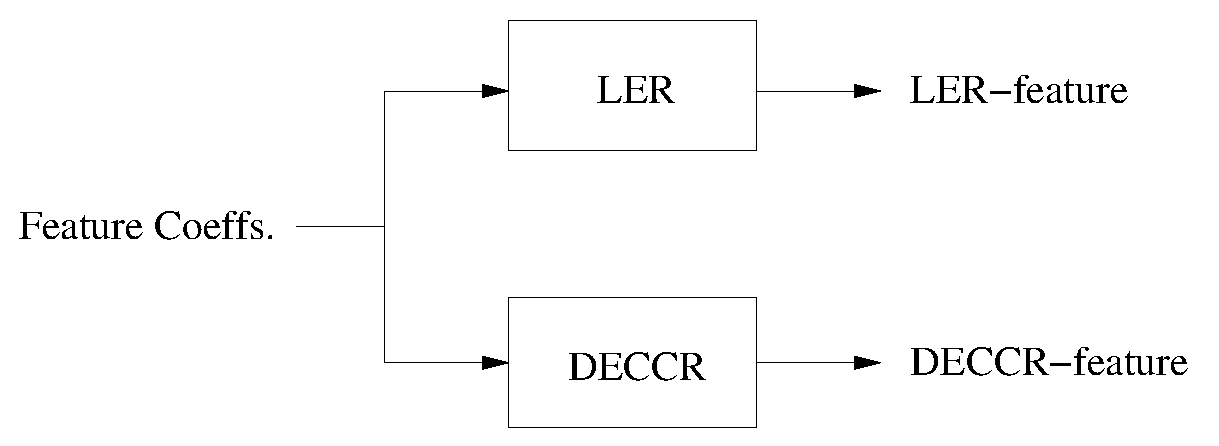
\includegraphics[width=1.0\textwidth]{figs/rescale}
\caption{重刻特徵參數流程圖} 
\label{fig:rescale}
\end{figure}

\section{資料驅動能量特徵重刻法}
\label{sec:ddt-rescaling}
能量特徵重刻在強健性語音辨識的領域中是屬於特徵補償的一種,
主要的目的是希望透過調整能量特徵以減少乾淨與含噪音特徵兩者的差異性。
我們觀察能量特徵的變化發現,一段雜訊語音中有語音的段落,其能量值偏高;反之,非語音的部分,能量值偏低。
基於此現象,本論文提出~DEFR~的方法對能量特徵作進一步的處理。

此方法主要分為語音活動偵測、分段對數尺度函數與參數搜尋法三個部分。
我們利用~\cite{tu2007}~所提出的低頻譜之語音活動偵測來取得語音與非語音出現的時間點,並利用分段對數尺度函數決定能量參數調整的權重值。
而分段對數尺度函數所使用的參數是由參數搜尋法自動決定。
以下我們就這三個部分做詳細說明。

\subsection{低頻譜之語音活動偵測}
\label{sec:vad}
在語音訊號處理系統中,語音訊號常常受到環境噪音的影響,使得系統效能低落。
因此發展了語音活動偵測來判斷訊號中語音與非語音的位置。
我們觀察語音在各個頻帶間能量的變化,發現無論任何種類的噪音,在頻帶~$\left[ 0,50 \text{Hz} \right]$~之間都有相當比例的能量。
藉由此特性,我們計算每個音框的低頻帶頻譜能量,並根據能量值,判斷該語音音框是否為純雜訊音框或是含語音的音框。
其做法詳細說明如下,首先假設我們有一段語句~(utterance)~$u$,對每個音框~$i$~取離散傅立葉轉換~(discrete Fourier transform, DFT),
式子為
\begin{equation}
\label{eq:dft}
	X^{(i)}(f_k) = X^{(i)}[k] = \sum_{n=0}^{N-1}x_i[n]e^{-j \frac{2 \pi kn}{K} }, 0 \leq k \leq K-1,
\end{equation}
其中~$f_k$~為頻率,其值為
\begin{equation}
	f_k = \frac{F_s}{2K}k,
\end{equation}	
其中~$F_s$~為取樣頻率,~$K$~為離散傅立葉的點數。在此
\[
	F_s = 8000, \quad K = 256.
\]
我們利用方程式(\ref{eq:dft})~可以得到每個頻率~$f_k$~的能量值,
因此我們定義頻帶~$\left[ F_L,F_H \right]$~之頻譜能量計算的方式為
\begin{equation}
\label{eq:energy_y}
	Y_{\left[ F_L,F_U \right]}^{(i)} = \sum_{F_L \leq f_k \leq F_U} \mid X_i \left( f_k \right) \mid.
\end{equation}
根據方程式(\ref{eq:energy_y}),我們計算每個音框之低頻帶頻譜強度,即~$0$~至~$50$Hz~以內的頻譜強度如下
\begin{equation}
	Y_{\left[ 0,50 \right]}^{(i)} = \sum_{ 0 \leq f_k \leq 50} \mid X_i \left( f_k \right) \mid.
\end{equation}
接著以一段語音前~$P$~個音框之低頻帶頻譜強度的平均為門檻值,其計算公式如下
\begin{equation}
	\label{eq:theta}
	\theta= \lambda \left( \frac{1}{P}\sum_{i=0}^{P-1} Y_{\left[ 0,50 \right]}^{(i)} \right),
\end{equation}
其中~$P$~為純噪音的音框數。
我們將每個音框低頻帶內的頻譜能量~$Y_{\left[ 0,50 \right]}^{(i)}$~與門檻值~$\theta$~做比較,
若~$Y_{\left[ 0,50 \right]}^{(i)} \leq \theta$~則將其歸類為非語音音框;反之,則屬於語音音框。
判斷式如下:
\begin{equation}
	\text{第$i$個音框} =  \begin{cases} Y_{\left[ 0,50 \right]}^{(i)} \leq \theta, &\text{非語音音框} \\   
					     Y_{\left[ 0,50 \right]}^{(i)} > \theta,&\text{語音音框}.
					\end{cases} 	
\end{equation}
VAD~的使用讓我們所提出之能量重刻的方法可以更加精確。
然而~VAD~的準確度對我們的實驗結果影響甚鉅,因此為了使~VAD~的準確度提高,
我們藉由改變方程式~(\ref{eq:theta})~中的~$P$~與~$\lambda$,使得~VAD~的準確度最佳化。
其中~$P$~與~$\lambda$~範圍設定如下
\[
	6 \leq P \leq 10, \quad 0.1 \leq \lambda \leq 2.0 .
\]
我們將強制對齊~(force alignment)~的方法實作在~Aurora 2.0~訓練語料庫,其實驗結果為語音與非語音訊號出現的時間點,
我們將此結果視為參考答案,接著與上述低頻帶能量之語音活動偵測器所得到的結果進行比對。
從實驗結果發現,當~$P = 10$~與~$\lambda = 1.9$~時~VAD~的準確率最高,其值如下表~\ref{table:vad_acc}。

\begin{table}[!htb]
\renewcommand{\arraystretch}{1.1}
\centering
\caption{低頻譜能量之語音活動偵測器的準確度}
\label{table:vad_acc}  
\vspace{2mm}
\begin{tabular}{cc}
\hline 
clean-train & multi-train  \\ 
\hline
{83.92} & {67.11}  \\
\hline
\end{tabular}
\end{table}

%{58.88} & {55.91} & {59.80}% \lamda = 1.9, P = 10
%{73.52} & 69.38 & 67.69 & 69.29 \\

\subsection{分段對數尺度函數}
\label{sec:piecewise}
分段對數尺度函數是為了使含語音的能量能夠確實地保留原有的能量值,
而非語音的能量能夠大幅度地下降,以增加語音與非語音能量的差異性。
首先,假設我們有一段語句~$u$~的特徵向量,
其處理過程如下
\begin{itemize}
\item 從每一語句~$u$~的~$c_0$~序列中找出最大~$c_0$~值~$M_u$~與最小~$c_0$~值~$m_u$。
\item 考慮每個音框~$i$~之特徵值~$c_0[i]$,定義~$r[i]$~為
  \[
	r[i] = \frac{c_0[i]-m_u}{M_u-m_u},
  \]
  很明顯地,我們會得到
  \[
  0 \le r[i] \le 1.
  \]
\item 進行重刻運算後的特徵為
  \begin{equation}
    \tilde c_0[i] = w[i] c_0[i],
  \end{equation}
  其中~$w[i]$~為音框~$i$~之權重。假設語句中的噪音屬於穩態的~(quasi-stationary),高能量的段落包含語音的可能性會相當高。
  因此,這意指
  \begin{equation}\label{eq:rescale}
    \begin{aligned}
      &r[i] \approx 1 \quad \longrightarrow \quad w[i] \approx 1, \\ 
      &r[i] \approx 0 \quad \longrightarrow \quad w[i] \approx 0.
    \end{aligned}
  \end{equation}
\end{itemize}
已經有很多方法實作方程式(\ref{eq:rescale})~的想法。
我們提出分段對數尺度函數實現上述的想法,函數為
\begin{equation}\label{eq:implementation}
  w[i] = \begin{cases} \left[ \frac{\log \left( r[i] \times M \right)}{\log \left( M \right)} \right]^{\alpha_1}, &Y_{\left[ 0,50 \right]}^{(i)} \le \theta \\  
    \left[ \frac{\log \left( r[i] \times M \right)}{\log \left( M \right)} \right]^{\alpha_2}, &Y_{\left[ 0,50 \right]}^{(i)} > \theta. 
  \end{cases} 
\end{equation}
其中~$Y_{\left[ 0,50 \right]}^{(i)}$~為~$0$~至~$50$~Hz頻譜的能量,$\theta$~為語音與非語音的門檻值。
方程式(\ref{eq:implementation})~中的參數~$M$~由經驗法則將其設定為~$100$,
而~$\alpha_1$~及~$\alpha_2$~是經由最小化平行語料庫之訓練集~(parallel training data sets)~整體的失真決定,
我們採用第~\ref{sec:algo}~節的參數搜尋法取得最佳的參數,其函數如圖~\ref{fig:ler}。
訓練與測試資料皆使用該參數進行能量重刻。

而~LER~與我們所提出之~DEFR~最大的差別在於~LER~權重的計算是使用對數轉換函數~(如圖~\ref{fig:logler}),其式子如下
\begin{equation}
\label{eq:lerweight}
	w[i] = \frac{\log \left( \left \lfloor r[i] \times M \right \rfloor \right)}{\log \left( M \right)}.
\end{equation}

我們以~LER~與~DEFR~調整~MFCC~與~TECC~的能量參數值,
其比較圖分別為圖~\ref{fig:testutt_mfcc}~與圖~\ref{fig:testutt}。
從圖中,我們可以很清楚地看出~MFCC~與~TECC~再重刻運算後,明顯地減少了乾淨與雜訊語句之差異。

\begin{figure}[!htb]
\centering
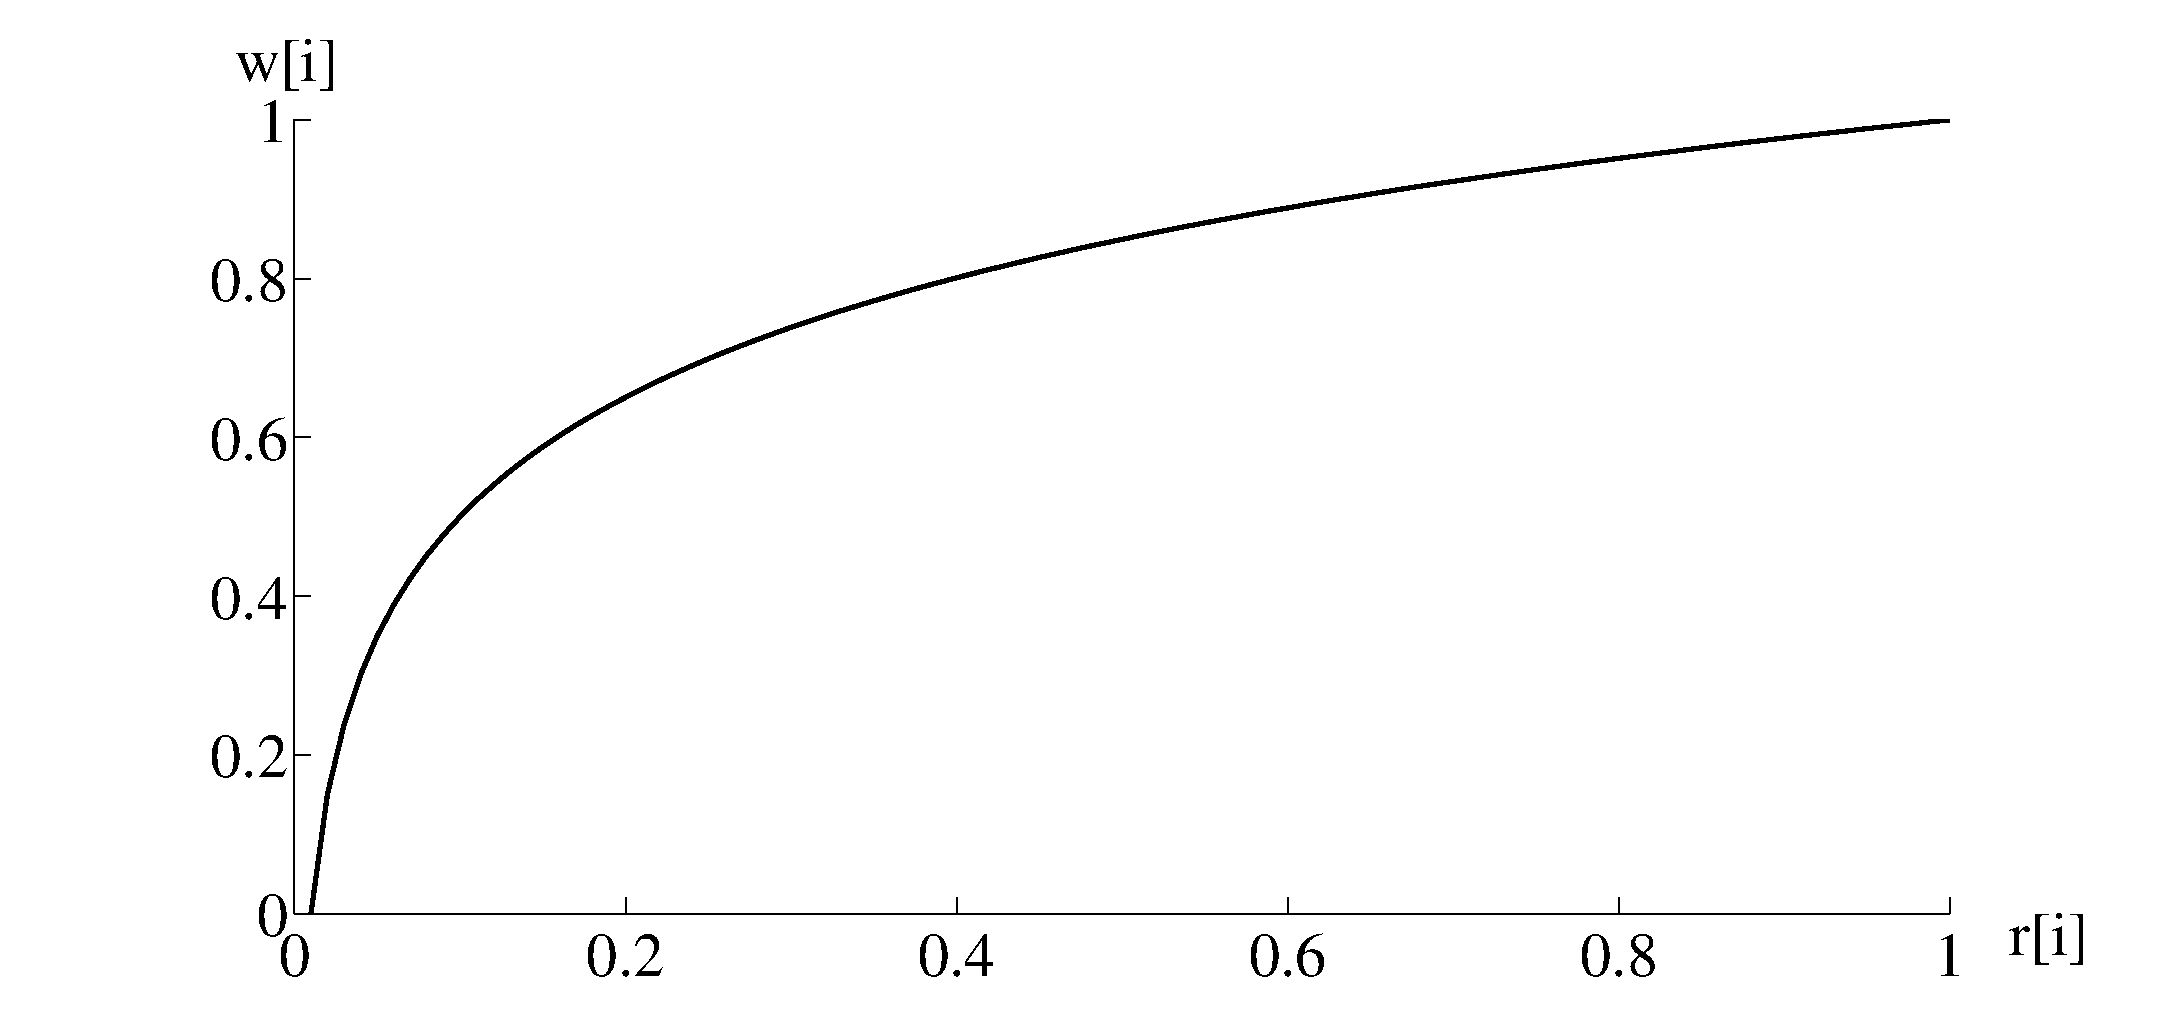
\includegraphics[width=0.8\textwidth]{figs/logler}
\caption{對數轉換函數} 
\label{fig:logler}
\end{figure}

\begin{figure}[!htb]
\centering
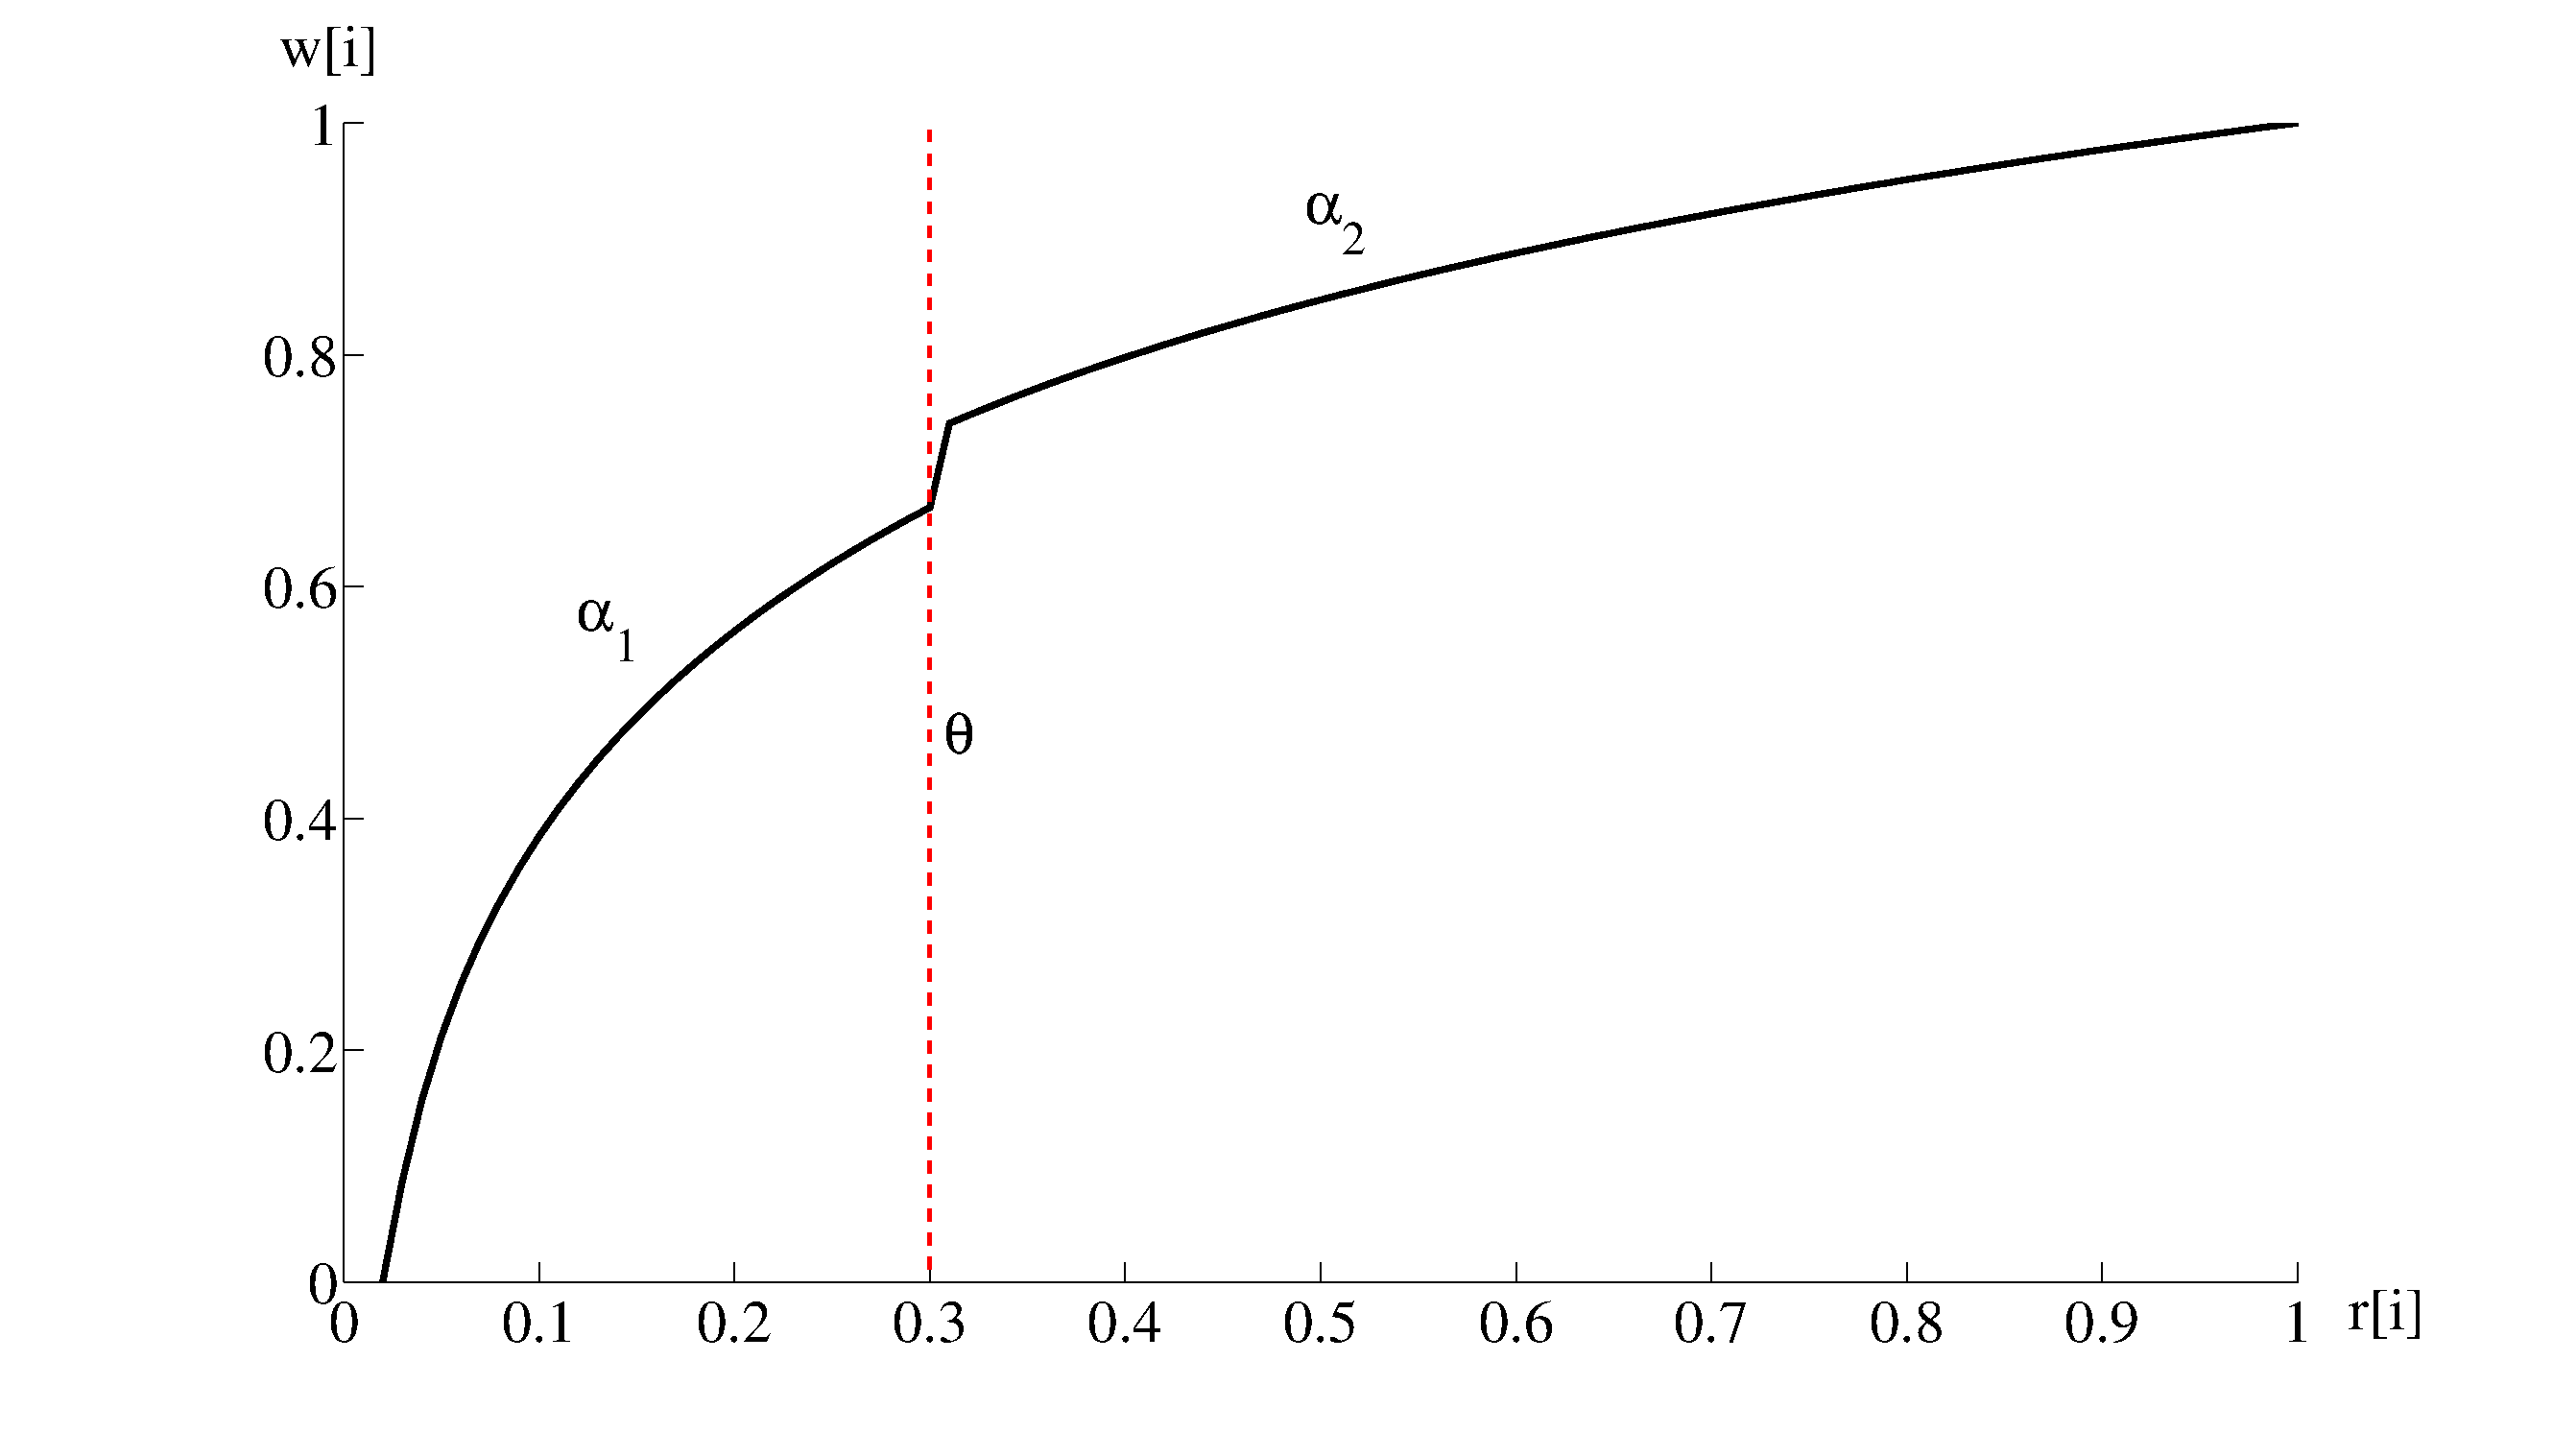
\includegraphics[width=1.0\textwidth]{figs/ler}
\caption{分段對數尺度函數。圖中~$\alpha_1$~和~$\alpha_2$~分別為非語音和語音能量所使用之參數} 
\label{fig:ler}
\end{figure}

\begin{figure}[!htb]
\centering
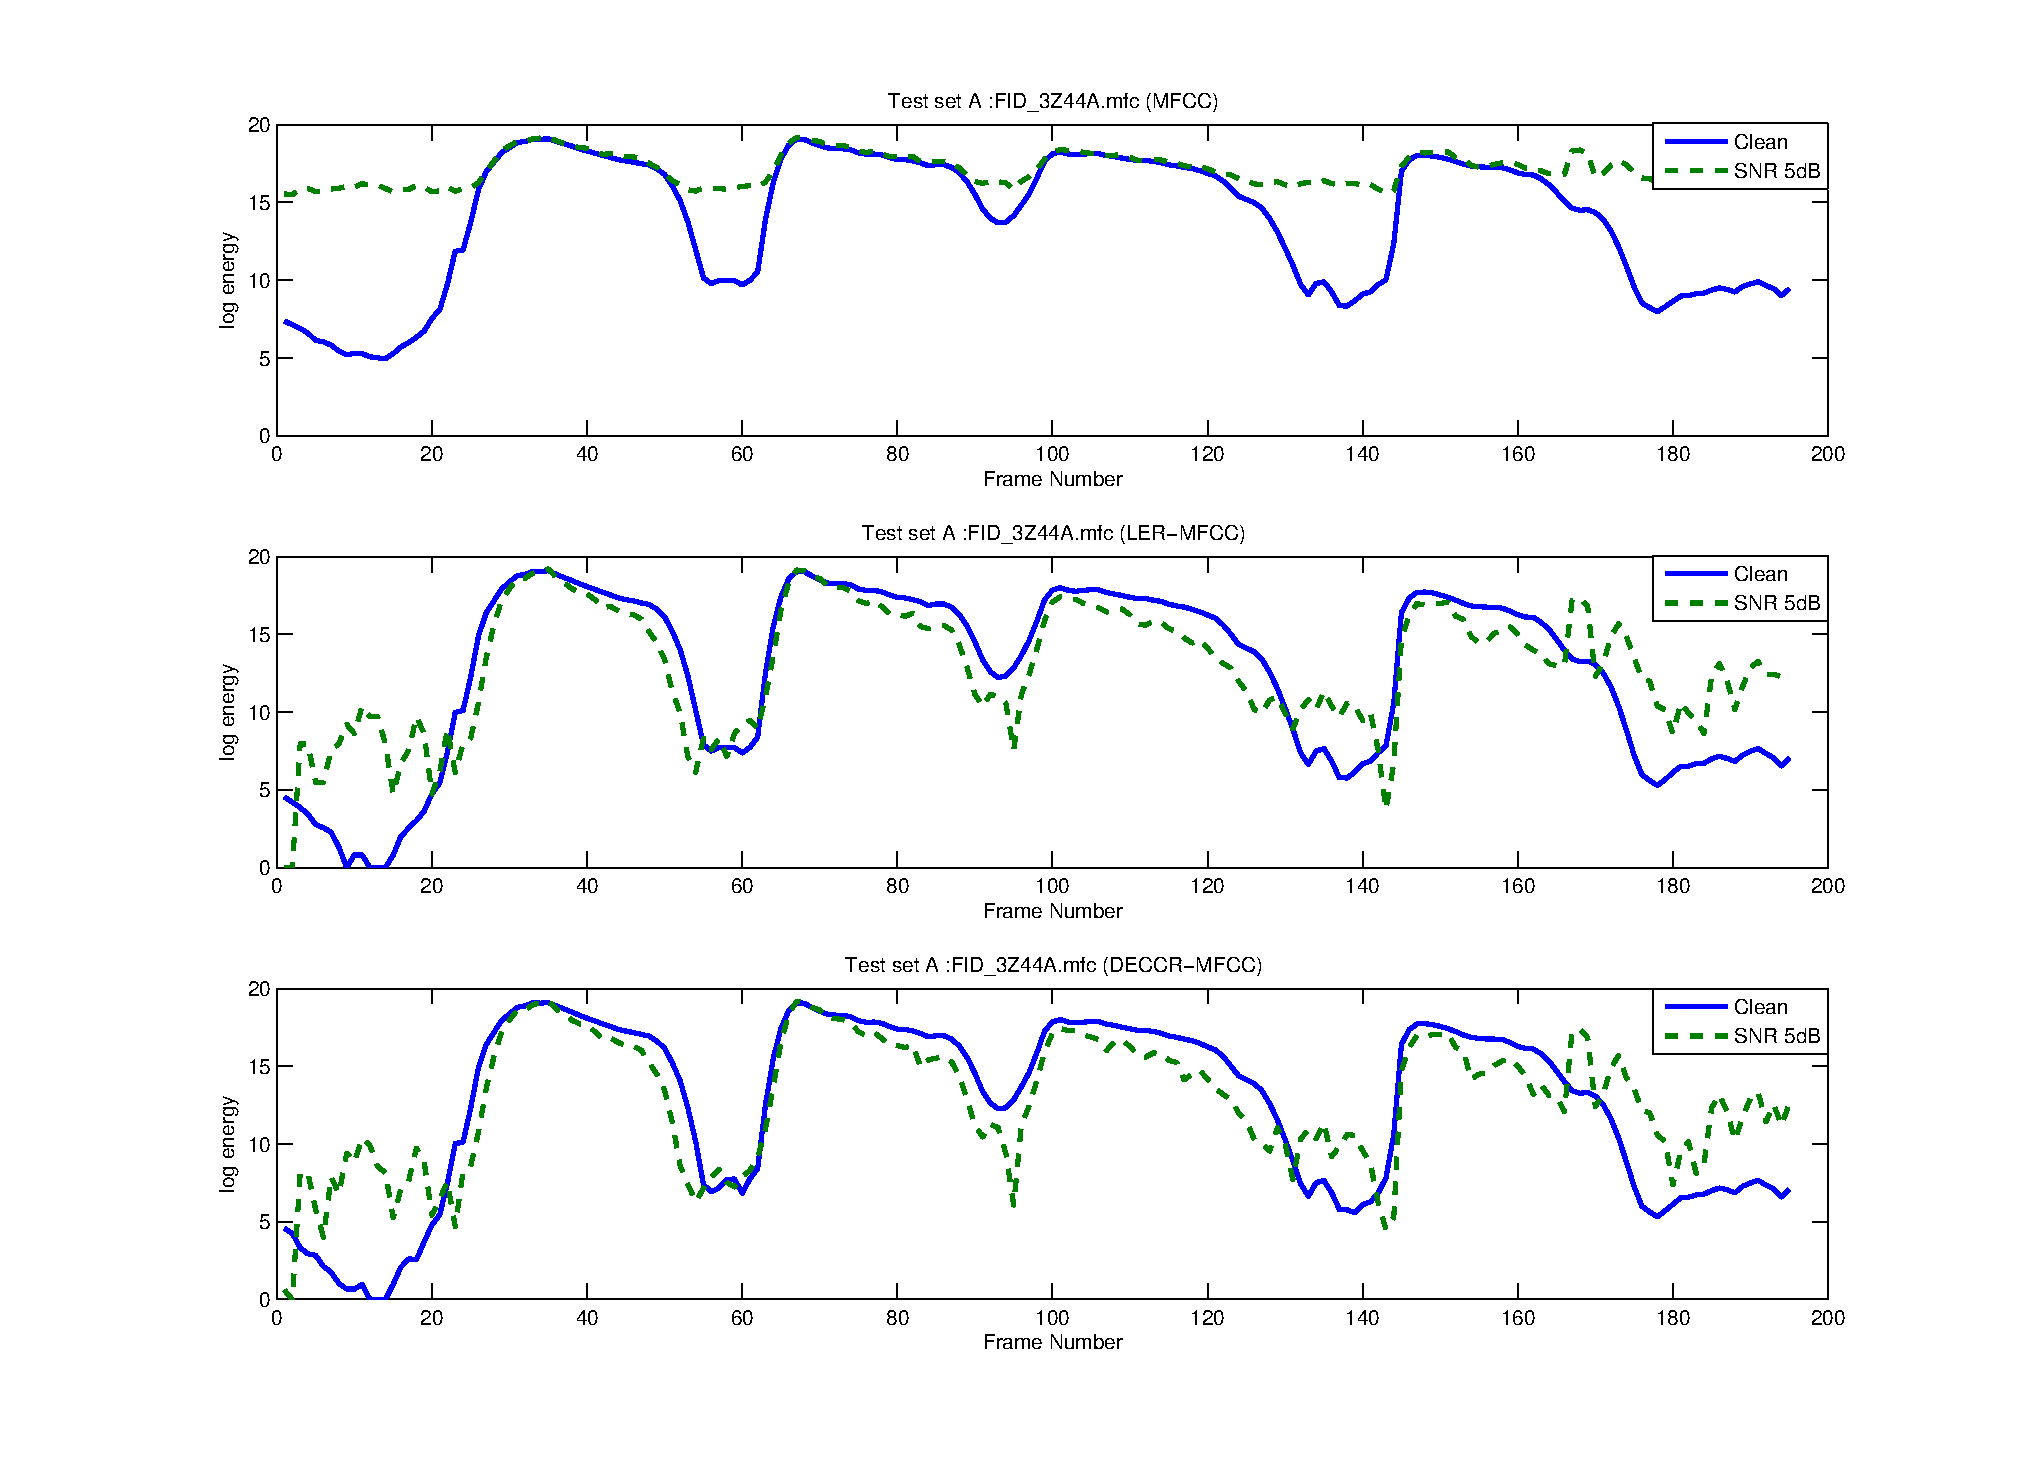
\includegraphics[width=1.0\textwidth]{figs/testutt_mfcc}
\caption{一對平行語句之~MFCC~(上)、LER-MFCC~(中)~與~DEFR-MFCC~(下)~對數能量序列的比較,語句的~ID~為~{\sffamily FID\_3ZZ4A.08}。} 
\label{fig:testutt_mfcc}
\end{figure}

\begin{figure}[!htb]
\centering
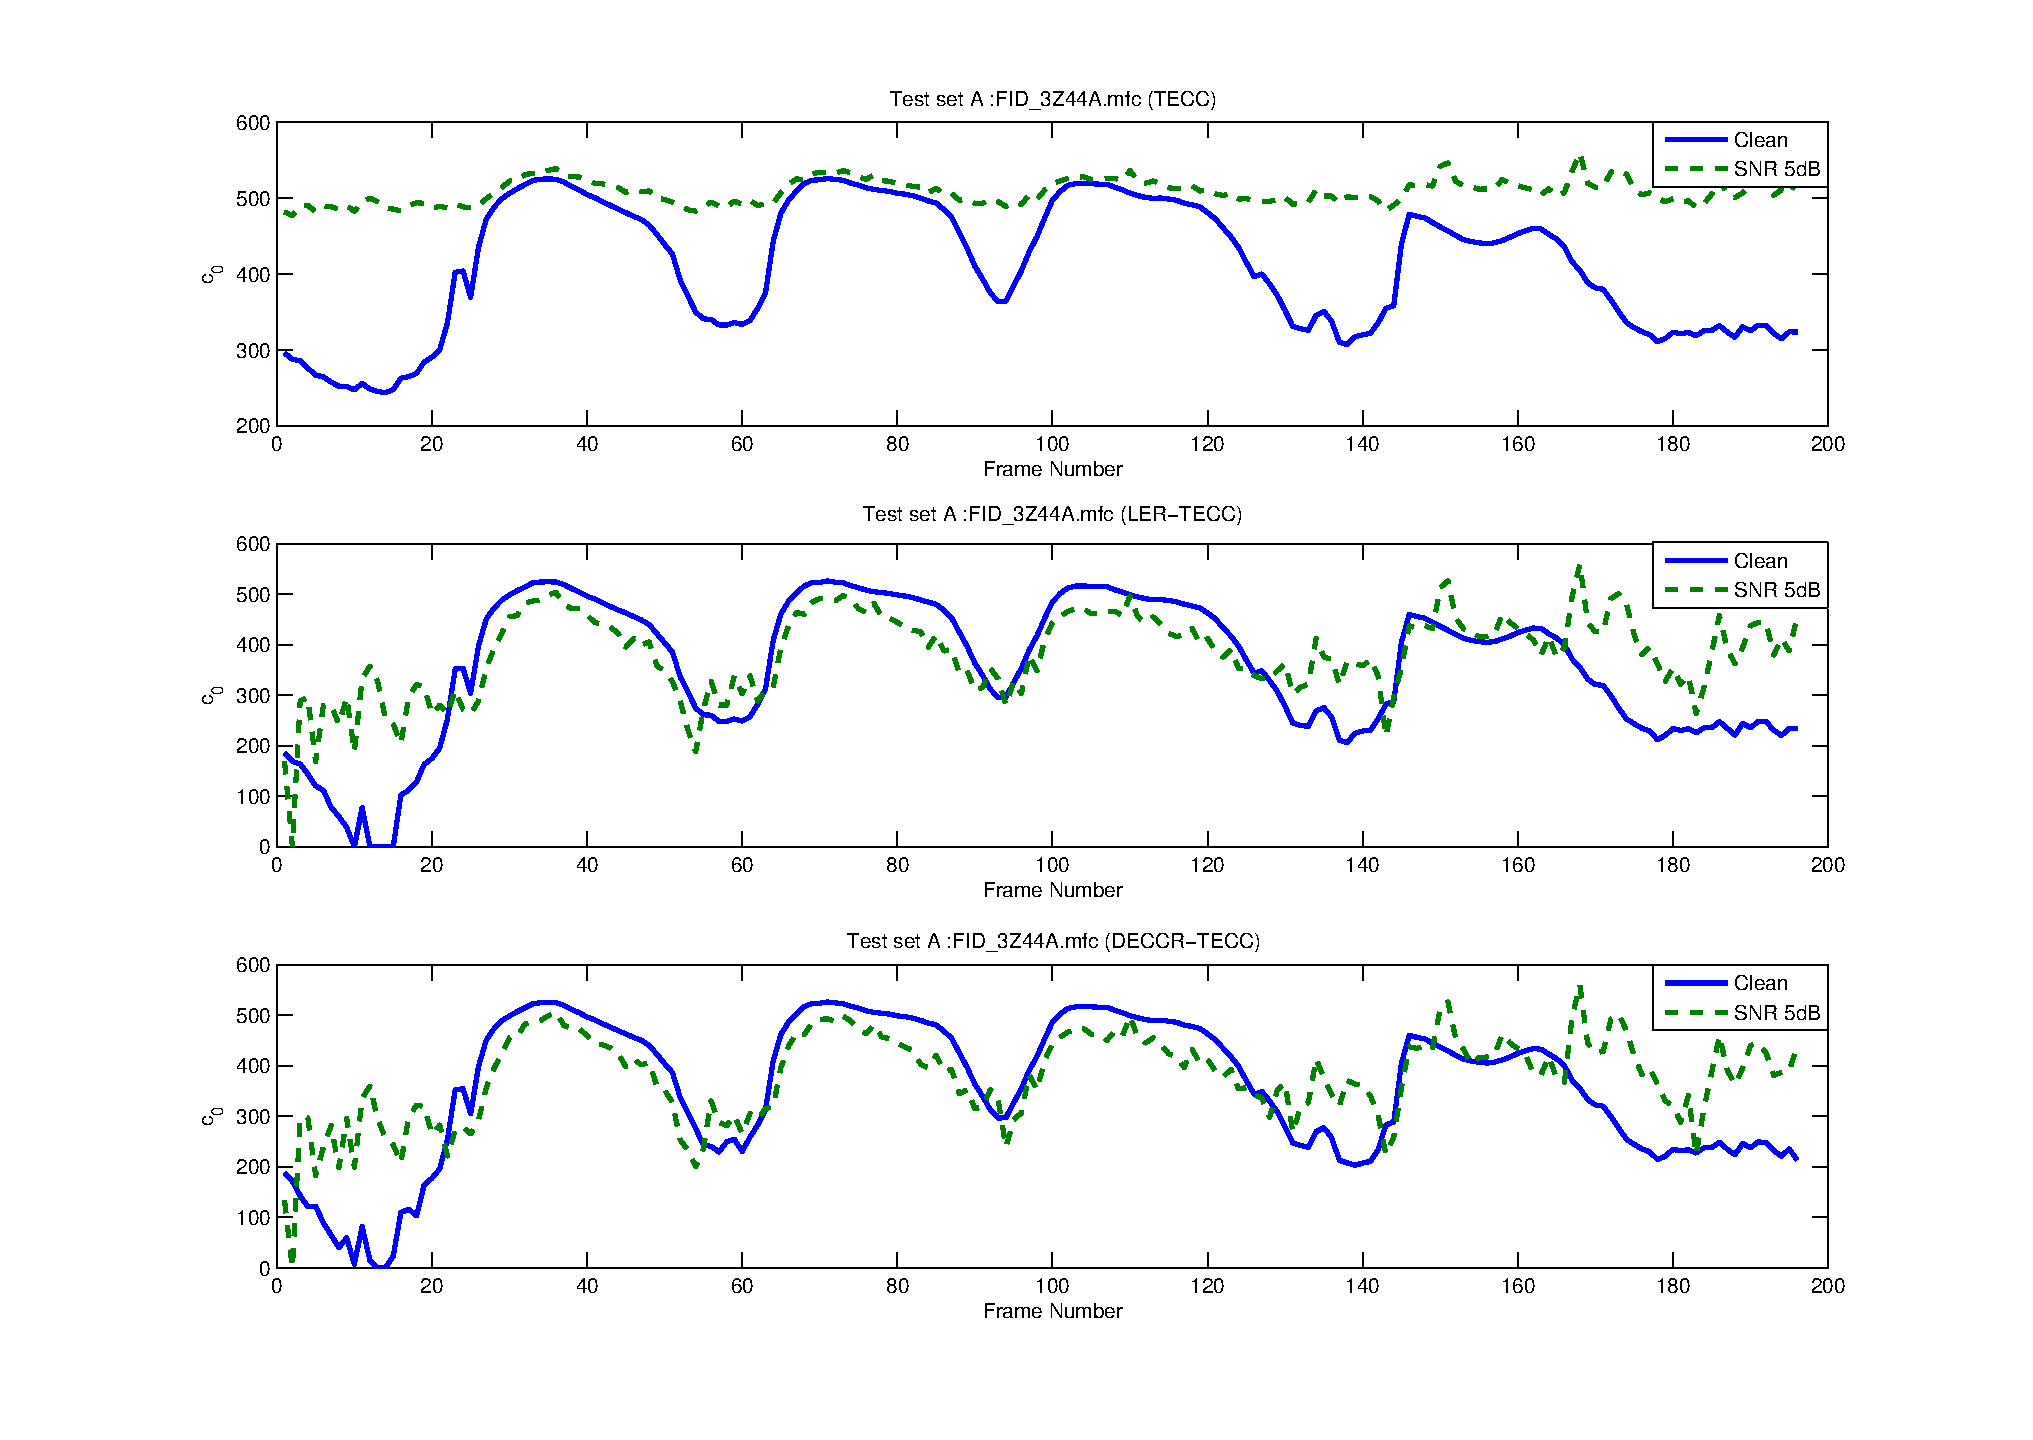
\includegraphics[width=1.0\textwidth]{figs/testutt}
\caption{一對平行語句之~TECC~(上)、LER-TECC~(中) 與~DEFR-TECC~(下)~$c_0$~特徵序列的比較,語句的~ID~為~{\sffamily FID\_3ZZ4A.08}。} 
\label{fig:testutt}
\end{figure}


\subsection{參數搜尋法}
\label{sec:algo}
本小節所提出的參數搜尋法,
目的為尋找第~\ref{sec:piecewise}~小節所使用之參數~$\alpha_1$~及~$\alpha_2$,
使得乾淨與雜訊語句特徵值的失真~(distortion)~最小化。
此方法必須滿足
\[
	1 \leq \alpha_2 < \alpha_1 \leq 2.
\]
我們希望非語音的特徵值可以快速下降,所以令~$\alpha_1 > \alpha_2$,使低於門檻值之特徵值下降速率提高。
而失真的計算方法如下式
\begin{equation}
\label{eq:distortion}
	D(\alpha_1, \alpha_2, \theta)= \sum_{u=1}^{U} \sqrt{\sum_{i=0}^{N-1} \left( N^u[i] - C^u[i] \right)^2 },
\end{equation}
其中~$U$~表示訓練語句的數目,$N$~表示語句~$u$~的音框數,
$C^u[i]$~與~$N^u[i]$~表示乾淨與含噪音語句~$u$~的第~$i$~個音框重刻後的特徵值。
